\section{Held-out and stress results}
V0, V1 and V5 produced identical navigation and calibration scores in every paired cell. V0 averaged $1.014^\circ$ yaw RMS versus $3.915^\circ$ with the sketch calibration switch off. The four-draw interval for that overall contrast crossed zero. Clean controls favored the opt-out ($0.255^\circ$ versus $0.428^\circ$). On distorted, uninterrupted records the corresponding means were $6.029^\circ$ and $1.208^\circ$.

V2/V3/V4 averaged $1.477/1.475/1.451^\circ$, and V6 averaged $3.186^\circ$. V6's worst paired increase was $10.346^\circ$. With weak excitation it stays close to identity, protecting clean records but retaining large installation errors. On development data, hard-only estimation had lower matrix Frobenius error than V0 (0.0094 versus 0.0109) and higher yaw RMS (1.205 versus 0.929 degrees).

V7 changed mean yaw RMS by $+0.0007^\circ$ (95\% interval $[-0.0103,+0.0116]^\circ$). V8 reduced the mean to $0.855^\circ$, improving 22 cells and degrading 10. Its worst increase was $0.0155^\circ$. All four draw-level means improved, by $0.114$ to $0.199^\circ$. For the ten-second bursts the mean fell from $1.212^\circ$ to $0.582^\circ$. V8 quarantined all 250 injected packets in each held-out burst and zero packets in the 24 clean or uninterrupted distorted records. Clean and uninterrupted combined means were essentially unchanged. Following/head means fell from $0.995/1.032^\circ$ to $0.817/0.894^\circ$. Mean 3-D displacement was 0.15288 m in V0 and 0.15269 m in V8; V6 increased it to 0.16682 m. The panel assigns a specified disturbance frequency that may differ from actual vessel operation.

V0 and V8 both gave mean per-axis applied offset RMS near $(0.262,0.249,0.223)\uT$. Mean posterior offset NEES was 1.51, with about 99.9\% of sampled offsets inside the nominal 95\% ellipsoid. Hard-only coverage was about 32\%. These repeated samples are correlated. The constrained model ignores multiplicative errors. We score a usable installation after 60 consecutive seconds with applied offset error below $1\uT$ and composite matrix Frobenius error below 0.03, starting at 180 s. V0/V8 qualified in 32/32 cells (median 240 s, latest 410 s); V6 qualified in 14/32. An initially good identity calibration can qualify without online learning. The first applied change has a separate score.

In the fixed-draw interference test, the maximum difference from a matched burst-free replay was $6.64/5.96^\circ$ (following/head) for V0 and $0.06/0.06^\circ$ for V8. V0 required 189/184 s after the burst before staying within $0.1^\circ$ for 10 s. V8 was already within that band. On the uninterrupted following-sea record, regression on time, 20 s steering quadratures and true roll/pitch gave a steering-harmonic amplitude of $0.0085^\circ$ for V0. Early (300--400 s) and late (1100--1200 s) signed means were $0.289^\circ$ and $1.069^\circ$. The sustained error changes more slowly than the commanded steering on this draw.

On the separate stress draw, 80 ms lag gave $4.092^\circ$ head-sea V8 RMS versus $4.094^\circ$ V0. Quarantine responds more readily to abrupt disturbances than to smooth timing error. During the larger maneuver, following/head RMS was $0.053/0.456^\circ$ for V0 and $0.051/0.452^\circ$ for V8; over the next 80 s it was $0.204/0.501^\circ$ and $0.197/0.496^\circ$. Engine and displaced-installation results also changed little. The CSVs preserve individual records, percentiles and worst regressions.

A post-hoc ablation removed the covariance adjustment while retaining the same six-microtesla gate and native calibration. Its mean yaw RMS was $0.856^\circ$; the change from V0 was $-0.158^\circ$ (four-draw interval $[-0.213,-0.103]^\circ$). All eight burst records improved and the other 24 were identical to V0. The interrupted mean was $0.581^\circ$. Mean 3-D error was 0.15269 m, with a worst paired increase of 0.00173 m. Worst paired roll RMS increased by $0.069^\circ$. Posterior matrix-error scores were unchanged. This ablation uses the native learner's qualified field prediction; the deployed sketch's opt-out cannot supply that prediction.

The successful intervention prevents rejected packets from reaching navigation and reference statistics. The trials establish no sustained calibration advantage during uninterrupted operation. We recommend retaining existing deployment defaults. A timestamped vessel or bench comparison with independent heading would be needed to quantify actual installation error, clock offset, false quarantine rate and board headroom.

\begin{figure*}[t]\centering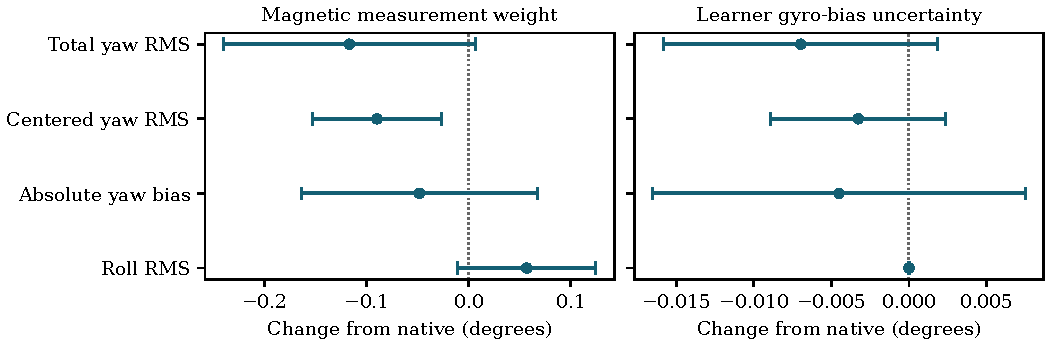
\includegraphics[width=.91\textwidth]{sustained-yaw.pdf}
\caption{Changes from the native setting on uninterrupted records. Each dot is a paired mean with its 95\% interval across independent sensor draws. Left, four draws testing stronger magnetic weight. Right, twelve further draws confirming the fourfold gyro-bias uncertainty setting. Negative changes correspond to lower error.}\end{figure*}

\section{Sustained heading without magnetic interference}
To test one alternative explanation, we changed the assumed magnetic standard deviation only after reference refinement. Each update uses the original live covariance multiplied by $k^2$. The learner, sensor packets, startup and 27-state dynamics remain identical. We scored 0.5, 1, 2 and 4 times native standard deviation on 12 uninterrupted development cells. At $k=0.5$ mean yaw RMS fell from $0.929$ to $0.871^\circ$, while roll RMS rose from $0.222$ to $0.276^\circ$. None of the three alternatives met the development requirements for yaw, absolute signed bias, roll/pitch and displacement. The lowest-yaw alternative was carried forward as a falsification test.

Four previously unused joint sensor draws (421, 829, 1609, 3517) supplied 32 paired PM--Stokes cells, all without interference, with both directions at 0.27, 1.5, 4 and 8.5 m. The 4 m cell used uninterrupted combined distortion. Mean yaw RMS fell from $0.707$ to $0.590^\circ$ ($-16.5\%$), improving 26 cells with six regressions and a worst increase of $0.138^\circ$. The paired four-draw 95\% interval for the change was $[-0.240,+0.006]^\circ$. Centered yaw RMS fell from $0.568$ to $0.479^\circ$ ($[-0.153,-0.027]^\circ$ for the change). Mean absolute within-record signed yaw bias fell from $0.324$ to $0.276^\circ$ with a change interval of $[-0.164,+0.068]^\circ$. Head-sea absolute bias improved from $0.494$ to $0.395^\circ$; following-sea bias moved from $0.154$ to $0.156^\circ$. These baseline means describe a distinct draw set.

Mean roll RMS rose from $0.180$ to $0.237^\circ$ ($+31.5\%$), with 27 regressions and a worst increase of $0.233^\circ$. Mean pitch RMS changed from $0.095$ to $0.097^\circ$ and 3-D displacement from 0.15384 to 0.15435 m. Near level attitude with field $(H,0,Z)$, the east component of a small rotation is $H\,\delta\psi-Z\,\delta\phi$, so the same magnetic residual can influence yaw and roll. This sensitivity experiment identifies a tradeoff in the full-vector update. It supplies no basis for a production-wide increase in magnetic weight.


\section{Gyro-bias uncertainty in the external learner}
Relative gyro rotation transports the local field between magnetic packets. We scaled the learner's initial gyro-bias standard deviation ($0.504$ mrad/s) and random-walk amplitude ($0.010$ mrad/s/$\sqrt{\mathrm s}$) together, keeping the navigation covariance and physical noise identical. On 12 development cells, fixing gyro bias at zero increased mean yaw RMS from $0.929$ to $9.370^\circ$. Even for clean magnetic inputs the four-cell average rose from $0.748$ to $9.812^\circ$. Across the 12 cells, mean posterior offset errors per axis grew from $(0.28,0.18,0.22)\uT$ to $(3.35,4.66,3.97)\uT$. The fitted matrix Frobenius error grew from 0.011 to 0.134. The fit can absorb angular-rate error into a spurious magnetic calibration.

At a quarter of the native standard deviations the development yaw RMS was $0.992^\circ$. A fourfold increase passed the development screen with $0.9286^\circ$ versus $0.9292^\circ$ native. Across four previously unused joint draws and 32 uninterrupted cases the fourfold setting reduced mean yaw RMS from $0.668$ to $0.656^\circ$ (25 improved, seven worsened, largest increase $0.012^\circ$). The paired 95\% change interval was $[-0.0204,-0.0026]^\circ$. Following/head means fell from $0.625/0.711^\circ$ to $0.613/0.699^\circ$. Mean absolute within-record bias changed by $-0.0126^\circ$ with interval $[-0.0260,+0.0007]^\circ$. Mean roll changed by $+0.00007^\circ$ and mean 3-D displacement by $-0.000007$ m.

We fixed the factor at four and repeated the comparison on 12 further independent sensor/initialization draws, eight physical conditions per draw. On these 96 pairs, mean yaw RMS was $0.7577^\circ$ native and $0.7507^\circ$ with the wider prior ($-0.92\%$). The draw-paired interval for the change was $[-0.0158,+0.0019]^\circ$. Fifty-three cells improved, 43 worsened and the largest increase was $0.044^\circ$. Mean absolute yaw bias changed from $0.5243^\circ$ to $0.5197^\circ$ (interval for the change $[-0.0165,+0.0075]^\circ$). Eight of the twelve draw-level total yaw means improved. Following/head yaw means moved from $0.7876/0.7277^\circ$ to $0.7771/0.7242^\circ$. On clean controls yaw rose from $0.4339$ to $0.4356^\circ$; on distorted records it fell from $0.8656$ to $0.8557^\circ$. Mean roll RMS changed by less than $0.00001^\circ$, mean 3-D displacement by $-0.000016$ m.

The seven stress fixtures in both directions averaged $1.0796^\circ$ native and $1.0786^\circ$ with the wider prior on their shared draw. The larger turn in head seas regressed from $0.753$ to $0.901^\circ$; both weak-steering records improved by about $0.033^\circ$. These results support retaining gyro bias in the external learner. Widening both its priors together failed the independent confirmation criteria for sustained yaw. The trials do not separate the initial bias variance from its random-walk rate.

\section{When does an installation need online correction?}
We crossed three magnetic inputs with three application policies on eight fresh joint draws. Each draw used all four PM--Stokes height/dip pairs in both directions. The ideal fixture supplies the exact body magnetic vector. The clean fixture adds white packet noise. The distorted fixture also includes the installation matrix, turn-on offset and offset random walk. Every arm consumes the same sensor random draws and uses the ordinary gyro, accelerometer and startup. Differences between fixtures therefore compare the indicated magnetic changes under matched motion and inertial errors.

The third policy (V11) lets the external estimator learn from the first eligible packet. It initially holds the applied correction at identity and zero offset. At five-second intervals it evaluates the estimated change in the noiseless field at the last posterior,
\[
 d=(\hat A-I)\hat f+\hat b,\qquad
 D=[\hat A-I,\ I,\ 0,\ \hat f^T\!\otimes I].
\]
It releases the native slew after three consecutive valid checks with $d^T(DPD^T)^{-1}d>16.27$, using all field, offset and matrix cross-covariances. The threshold and persistence were fixed before these replays. The repeated posterior scores are correlated, so the threshold serves as a decision rule and has no assigned record-level false alarm probability. After release the learner follows the usual application policy for the remainder of the record.

Across the 64 matched conditions, native learning reduced mean yaw RMS on distorted inputs from $3.341$ to $0.898^\circ$ (paired 95\% change interval $[-3.717,-1.170]^\circ$). On clean, noisy inputs it increased yaw RMS from $0.469$ to $0.765^\circ$ ($[+0.108,+0.484]^\circ$). With learning disabled, white packet noise changed the ideal-input mean by only $+0.001^\circ$. With learning enabled, the same noise changed it by $+0.278^\circ$. The within-draw difference of those two effects was $+0.277^\circ$ ($[+0.068,+0.485]^\circ$). White packet noise can therefore create a sustained heading penalty through online calibration even with no true offset or gain error. Residual yaw with ideal packets and learning disabled averaged $0.468^\circ$, reaching $0.984^\circ$ on the 8.5 m/$76^\circ$ condition. Height and inclination vary together in this panel.

V11 withheld the correction throughout all 64 clean noisy records, reducing mean yaw RMS from $0.765$ to $0.469^\circ$ relative to V0 ($-38.7\%$). On distorted records V11 released in 62/64 cases, at a median of 65 s among releases. Mean yaw RMS moved from $0.898$ to $0.907^\circ$ (paired change $+0.009^\circ$, interval $[-0.042,+0.061]^\circ$). Both missed releases were in 0.27 m waves. The worst regression also occurred in that sea, on a different record. Release at 745 s raised the head-sea RMS from $0.541$ to $1.724^\circ$. Delaying until the distortion is well resolved can leave a real heading error in place for much of the scoring window.

\begin{figure*}[t]\centering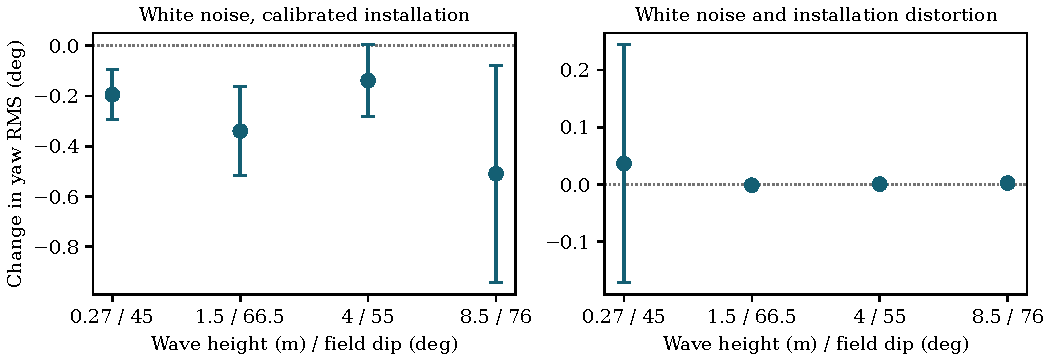
\includegraphics[width=.93\textwidth]{installation-screen.pdf}
\caption{Change in yaw RMS when applying the installation screen instead of always-on calibration. Each point averages the paired effects across both directions within each of eight independent draws. Bars show two-sided 95\% intervals across those draws. The vertical scales differ.}\end{figure*}

\begin{table}[t]\centering\footnotesize
\caption{Mean yaw RMS in degrees for opt-out, native continuous calibration and screened application. The last column counts records in which V11 released the correction.}
\begin{tabular}{llrrrr}\toprule
Panel & Input & Off & Native & V11 & Released\\\midrule
Four seas & Ideal & 0.468 & 0.487 & 0.468 & 0/64 \\
Four seas & Clean & 0.469 & 0.765 & 0.469 & 0/64 \\
Four seas & Distorted & 3.341 & 0.898 & 0.907 & 62/64 \\
0.27 m & Ideal & 0.377 & 0.368 & 0.377 & 0/32 \\
0.27 m & Clean & 0.392 & 0.624 & 0.392 & 0/32 \\
0.27 m & Distorted & 3.433 & 0.778 & 0.801 & 32/32 \\
\bottomrule
\end{tabular}\end{table}

We then fixed the 0.27 m record, crossed magnetic dips of $45^\circ$ and $76^\circ$ in both directions, and repeated the nine arms on eight independent new draws (288 replays). On 32 clean noisy records the screen again withheld every correction. Mean yaw RMS fell from $0.624$ to $0.392^\circ$ relative to V0 (paired change $-0.232^\circ$, interval $[-0.448,-0.016]^\circ$). The interval for the change in absolute within-record signed bias included zero on both panels. On distorted weak-wave records the screen released in all 32 cases, at median 112.5 s. Mean yaw RMS moved from $0.778$ to $0.801^\circ$ ($+0.023^\circ$, interval $[-0.011,+0.057]^\circ$). Even with eventual detection, a 375 s release raised one head-sea RMS from $0.226$ to $0.633^\circ$. Across the distorted cases the maximum paired increases in roll and pitch RMS stayed below $0.001^\circ$ on both panels. These results support screening as a way to protect an already calibrated installation in simulation. They give no sustained-yaw advantage over native learning when actual distortion is present. The release delays and absence of vessel trials limit deployment.

The fixed stress draw covered engine vibration, displaced mounting, magnetic latency, outliers, a low--high--low sea transition, weaker steering and a larger turn in both directions. The screen released between 40 and 80 s in all 14 records, before the ordinary post-refinement correction became eligible. All 14 sustained yaw scores matched V0. These records exercise the early-release path and give limited information about disturbances that start while a correction is still withheld.
